\subsection{Airframe Concepts}

As stated in Section \ref{sec:Concept_Generation_Approach}, an iterative approach was used to generate and improve upon airframe concepts. The following sections detail a selection of concepts from each round of analysis.

\subsubsection{Round 1 Concepts}
% Show the basic images of the desings
%include description and advantages/disadvantages in appendix (similar to ATLAS report) 
% Include the performance score and the visual displaying strengths and weaknesses
% * This section will show CAD drawings and radar charts of selected concepts. An example of the layout (minus a CAD drawing) is given below.\\
\note{Rhys}{1-[Rhys],5-[Jake],6-[Peter],12-[Sam],8-[Harry]}\\
\note{Rhys}{Actually show/visualise score for each desing}\\
\note{Rhys}{Make a note why objective 2 and 7 arnt in this analysis}\\
\note{Rhys}{Round 1=6 designs. Round 2=4 designs. Round 3=2 designs}\\

\paragraph{Concept 1: Commercially Available VTOL UAV}
This fixed wing fuselage UAV features a channelled wing design to promote more lift at low speeds and therefore reduce stall speeds. The four motors for hover and VTOL capabilities allow for high stability as they are placed away from the centre line and therefore produce a larger moment to counter disturbances. One horizontal pusher motor is used in forward flight, simplifying transition as no motor rotation is required. This leads to inefficiencies however as during both flight modes there are motors that are not active and are essentially dead weight. Due to the channelled wing, manufacturing complexity is increased. Figure \ref{fig:concept1} shows the concept and its performance criteria assessment results. 



\begin{figure}[H]
\centering
\begin{subfigure}[t]{.5\textwidth}
  \centering
  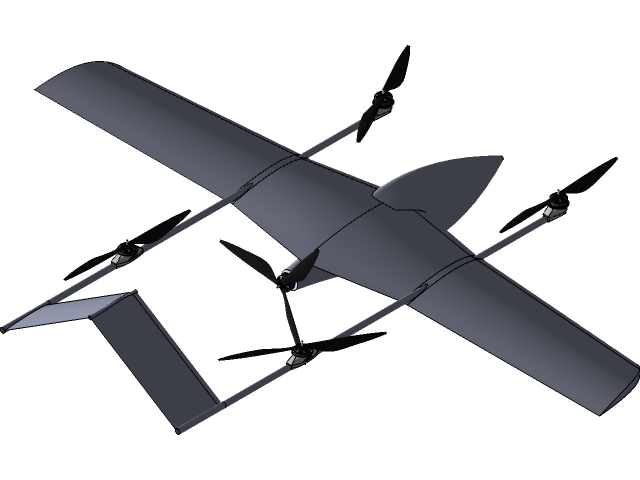
\includegraphics[width=0.85\linewidth]{Concepts/CAD/1cad.png}
  \caption{CAD Drawing}
  \label{fig:cad1}
\end{subfigure}%
\begin{subfigure}[t]{.5\textwidth}
  \centering
  \fbox{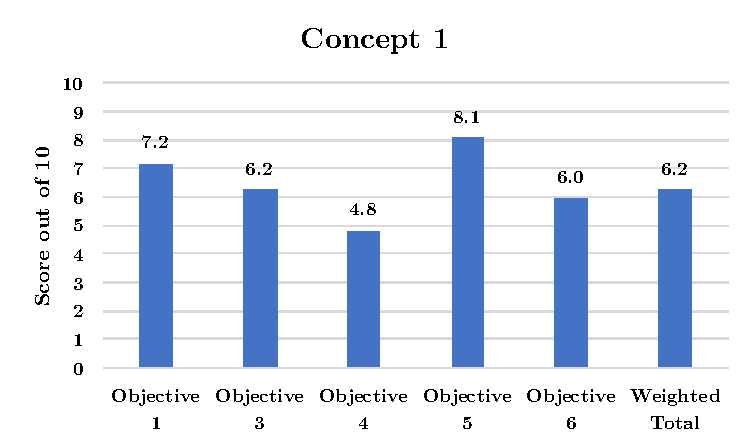
\includegraphics[width=0.95\linewidth]{Concepts/Plots/1.pdf}}
  \caption{Performance Criteria Assessment Results}
  \label{fig:radar1}
\end{subfigure}
\caption{Concept 1: Commercially Available VTOL UAV}
\label{fig:concept1}
\end{figure}


\paragraph{Concept 2: Bi-wing Tailsitter}
\note{Tom}{Change from bi-wing to reflect Jake's design}
This bi-wing tailsitter uses a large diameter propeller for propulsion and two smaller propellers mounted perpendicularly for stabilisation. The large diameter of the main propeller increases efficiency in both hover and forward flight modes, but the large wetted area causes significant amounts of drag at high speeds. The system does not require any moving parts other than the motors, therefore reducing manufacturing complexity. Due to the nature of tailsitters, the payload is not oriented in the same plane during all flight modes. This design therefore requires additional systems such as gimbals or extra sensors to maintain a consistent relevant data feed from the payload. Figure \ref{fig:concept2} shows this design and its performance.



\begin{figure}[H]
\centering
\begin{subfigure}[t]{.5\textwidth}
  \centering
  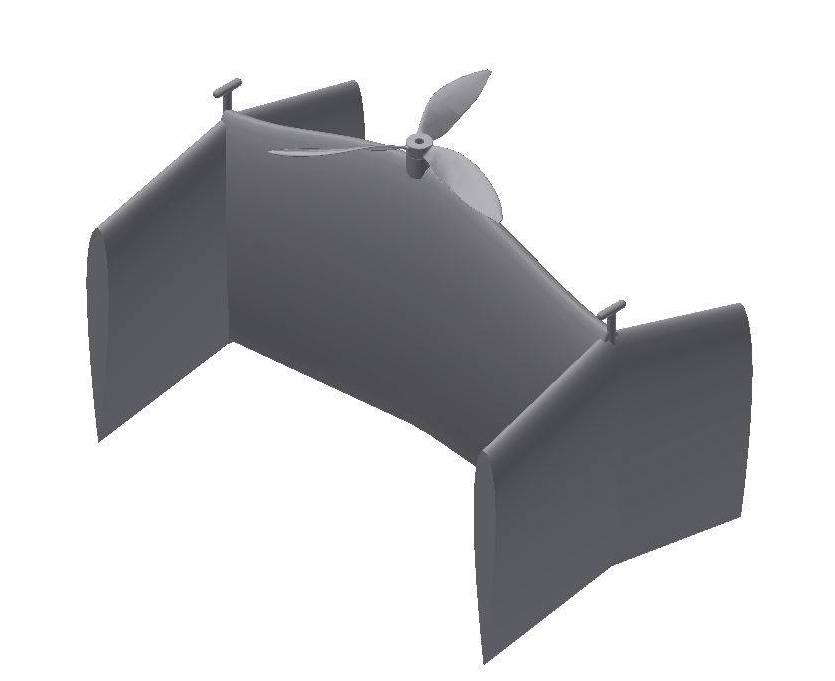
\includegraphics[width=0.75\linewidth]{Concepts/CAD/5cad.jpg}
  \caption{CAD Drawing}
  \label{fig:cad2}
\end{subfigure}%
\begin{subfigure}[t]{.5\textwidth}
  \centering
  \fbox{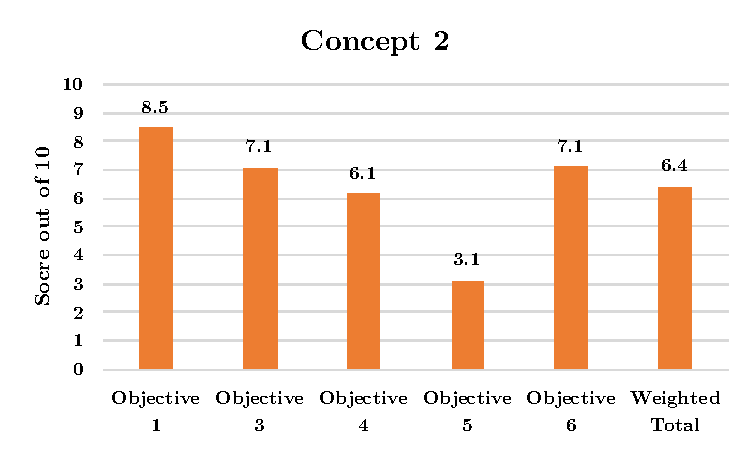
\includegraphics[width=0.95\linewidth]{Concepts/Plots/5.pdf}}
  \caption{Performance Criteria Assessment Results}
  \label{fig:radar2}
\end{subfigure}
\caption{Concept 2 - Bi-wing Tailsitter}
\label{fig:concept2}
\end{figure}


\paragraph{Concept 3: Distributed Lift Tilt Wing}
This concept leverages the increased efficiency from distributed propulsion over the main wing in both forward flight and hover modes by incorporating a wing tilting mechanism. Efficiency will can be further increased by overlapping the propellers and adding the ability to deactivate motors to reduce power consumption if required. A tilt tail pusher is included to add stability in hover modes while also adding thrust during forward flight. Figure \ref{fig:concept3} shows this design and its performance.

% Tilt-wing, distributed lift design with a tilt tail pusher. Wing is integrated into main fuselage, housing tilting mechanism. Pusher tilt mechanism is housed in the rear of the fuselage.  Main lift system is the distributed lift over the wing, using smaller but more efficient motors and by overlapping disk areas of props will increase efficiency of lift generation. Can possibly include a system to deactive certain motors on the wing to save power if required. 

\begin{figure}[H]
\centering
\begin{subfigure}[t]{.5\textwidth}
  \centering
  \fbox{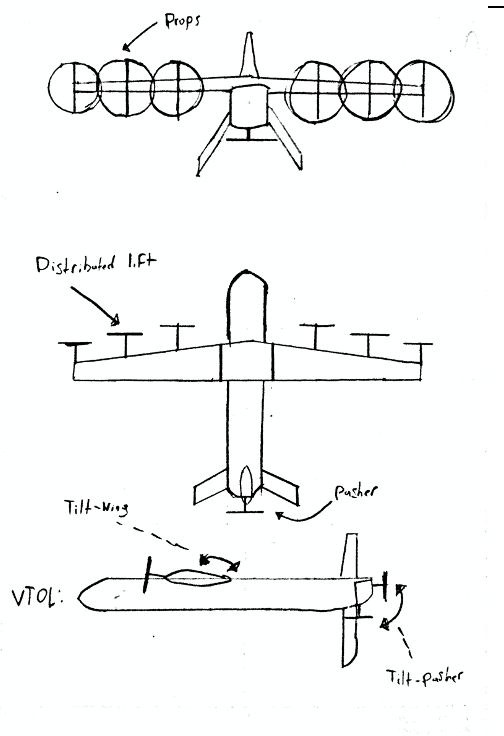
\includegraphics[width=0.95\linewidth]{Concepts/CAD/6.png}}
  \caption{CAD Drawing}
  \label{fig:cad3}
\end{subfigure}%
\begin{subfigure}[t]{.5\textwidth}
  \centering
  \fbox{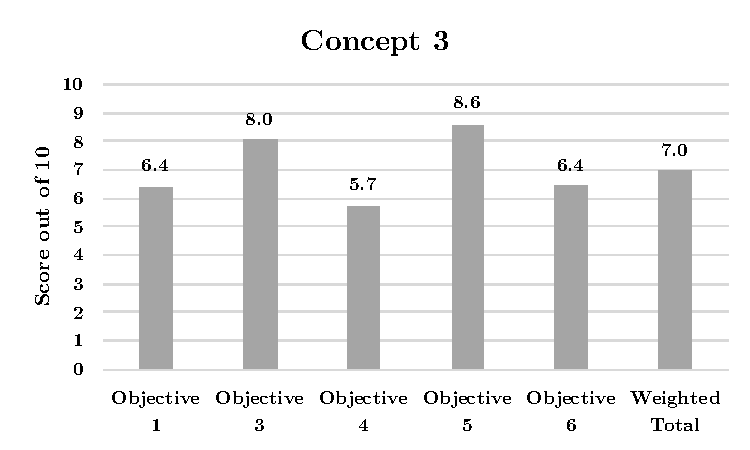
\includegraphics[width=0.95\linewidth]{Concepts/Plots/6.pdf}}
  \caption{Performance Criteria Assessment Results}
  \label{fig:radar3}
\end{subfigure}
\caption{Concept 3 - Commercially Available VTOL UAV}
\label{fig:concept3}
\end{figure}

\begin{figure}[H]
\centering
\begin{subfigure}[t]{.5\textwidth}
  \centering
  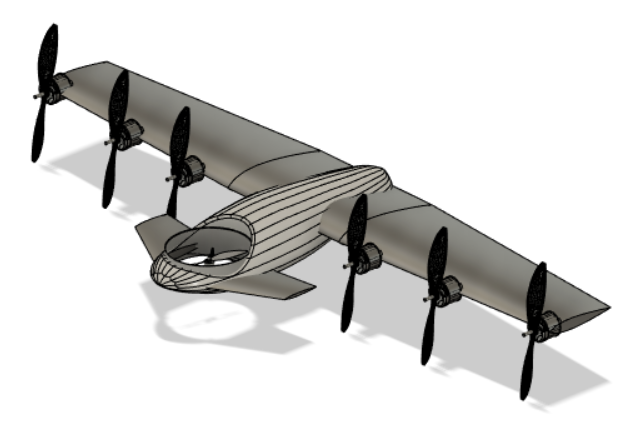
\includegraphics[width=0.95\linewidth]{Concepts/CAD/8cad.png}
  \caption{CAD Drawing}
  \label{fig:cad1}
\end{subfigure}%
\begin{subfigure}[t]{.5\textwidth}
  \centering
  \fbox{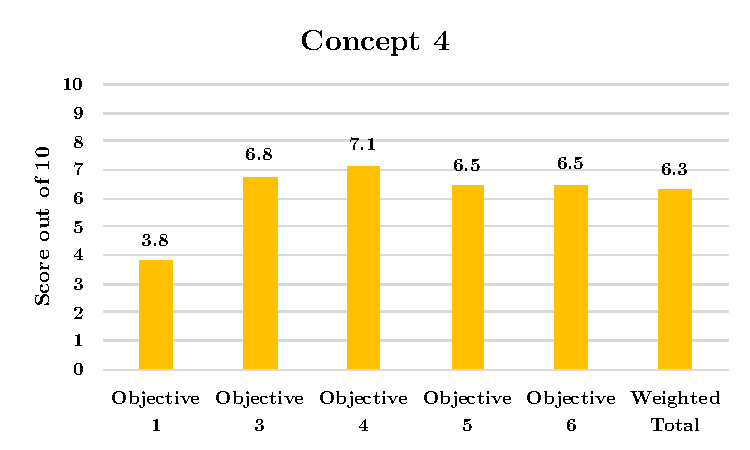
\includegraphics[width=0.95\linewidth]{Concepts/Plots/8.pdf}}
  \caption{Performance Criteria Assessment Results}
  \label{fig:radar1}
\end{subfigure}
\caption{Concept 4 - Commercially Available VTOL UAV}
\label{fig:concept2}
\end{figure}

\begin{figure}[H]
\centering
\begin{subfigure}[t]{.5\textwidth}
  \centering
  \fbox{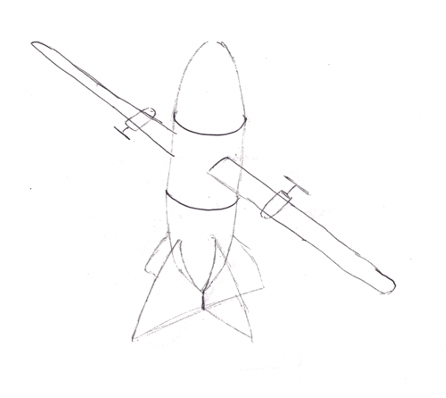
\includegraphics[width=0.95\linewidth]{Concepts/CAD/12.png}}
  \caption{CAD Drawing}
  \label{fig:cad1}
\end{subfigure}%
\begin{subfigure}[t]{.5\textwidth}
  \centering
  \fbox{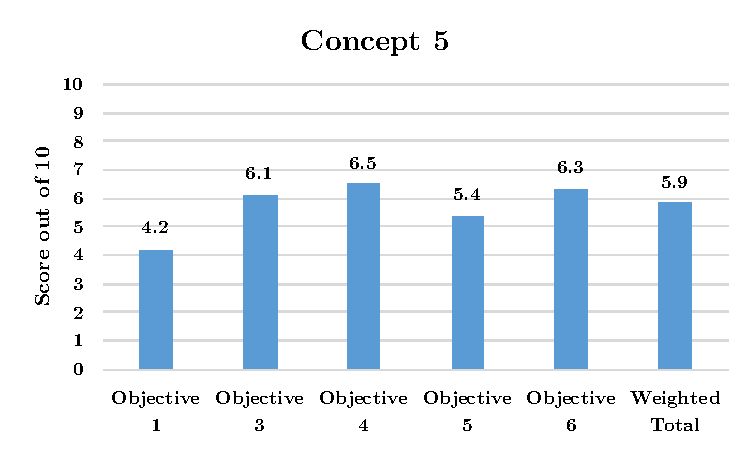
\includegraphics[width=0.95\linewidth]{Concepts/Plots/12.pdf}}
  \caption{Performance Criteria Assessment Results}
  \label{fig:radar1}
\end{subfigure}
\caption{Concept 5 - Commercially Available VTOL UAV}
\label{fig:concept2}
\end{figure}

*A summary visual will also be provided to help compare between the concepts.
\begin{figure}[H]
    \centering
    \fbox{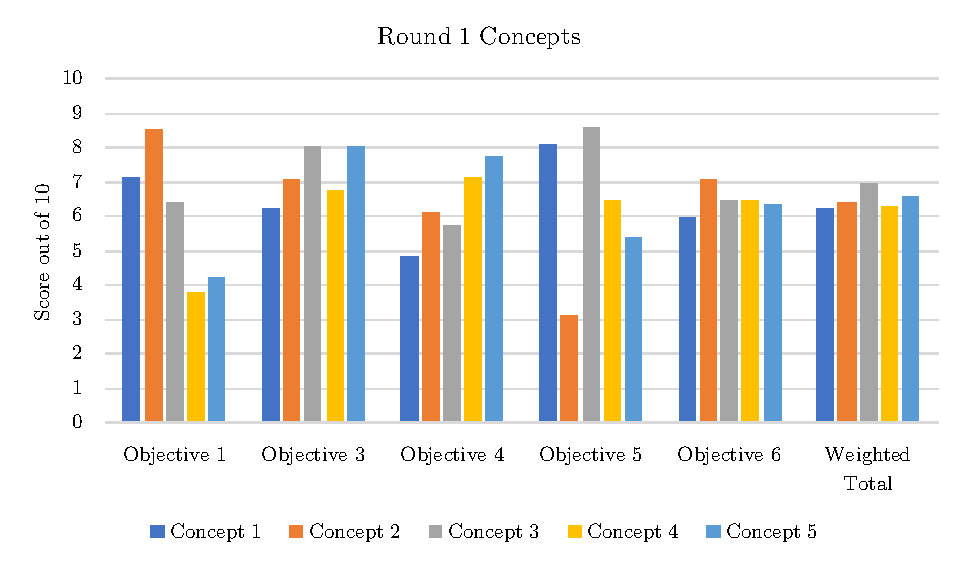
\includegraphics[width = \textwidth]{Concepts/Plots/Round1.pdf}}
    \caption{Summary of Design for Objectives evaluation and scoring for Round 1 Concepts}
    \label{fig:summary}
\end{figure}

\note{Peter}{switch objectives and concepts}

* Further description of each concept will be displayed in the appendix. 


\subsubsection{Round 2 Concepts}
similar to round 1 concepts
\note{Rhys}{5-[Peter],6-[Harry],7-[Jake]}


\begin{figure}[H]
\centering
\begin{subfigure}[t]{.5\textwidth}
  \centering
  \fbox{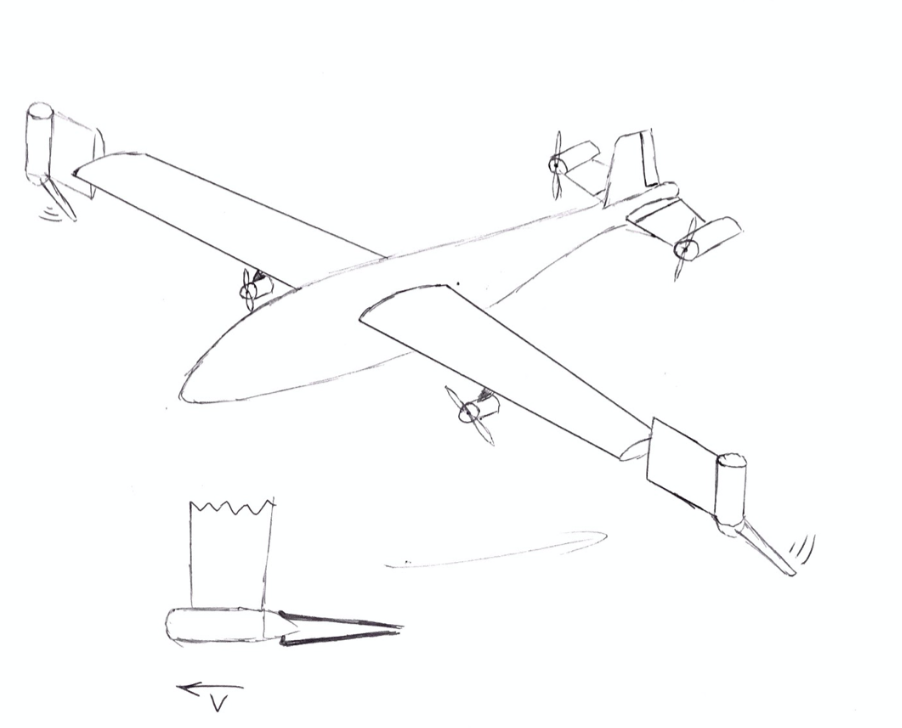
\includegraphics[width=0.95\linewidth]{Concepts/CAD/Round2_1.png}}
  \caption{CAD Drawing}
  \label{fig:cad1}
\end{subfigure}%
\begin{subfigure}[t]{.5\textwidth}
  \centering
  \fbox{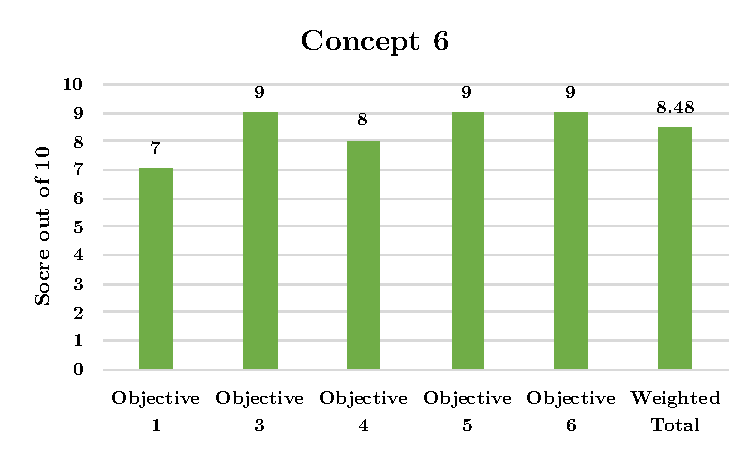
\includegraphics[width=0.95\linewidth]{Concepts/Plots/Round2_1.pdf}}
  \caption{Performance Criteria Assessment Results}
  \label{fig:radar1}
\end{subfigure}
\caption{Concept 5 - Commercially Available VTOL UAV}
\label{fig:concept2}
\end{figure}




\begin{figure}[H]
\centering
\begin{subfigure}[t]{.5\textwidth}
  \centering
  \fbox{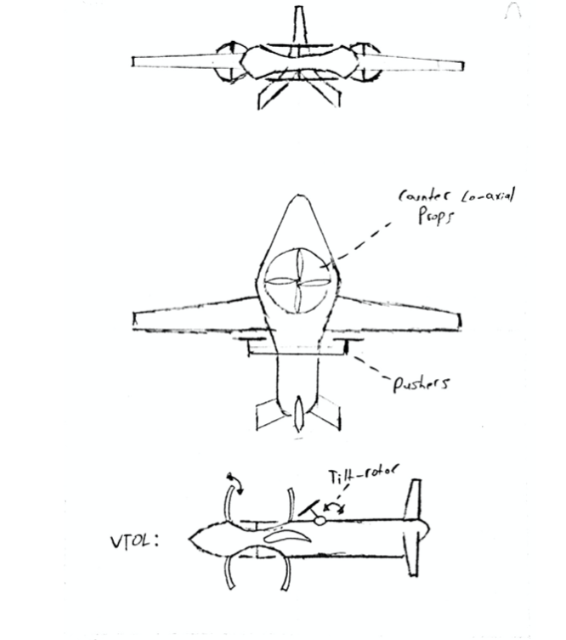
\includegraphics[width=0.95\linewidth]{Concepts/CAD/Round2_2.png}}
  \caption{CAD Drawing}
  \label{fig:cad1}
\end{subfigure}%
\begin{subfigure}[t]{.5\textwidth}
  \centering
  \fbox{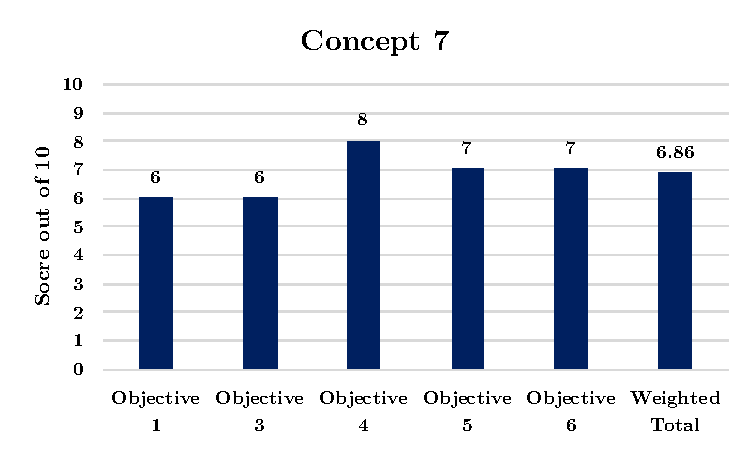
\includegraphics[width=0.95\linewidth]{Concepts/Plots/Round2_2.pdf}}
  \caption{Performance Criteria Assessment Results}
  \label{fig:radar1}
\end{subfigure}
\caption{Concept 5 - Commercially Available VTOL UAV}
\label{fig:concept2}
\end{figure}




\begin{figure}[H]
\centering
\begin{subfigure}[t]{.5\textwidth}
  \centering
  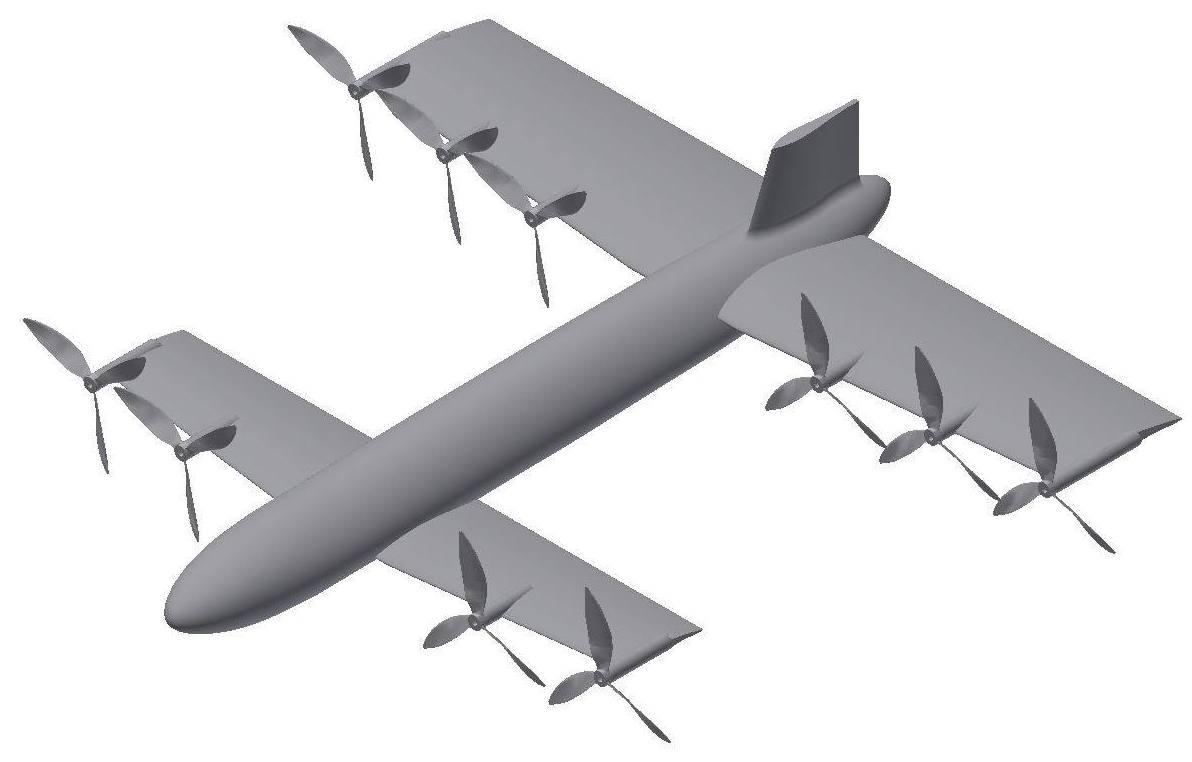
\includegraphics[width=0.95\linewidth]{Concepts/CAD/Round2_3_cad.jpg}
  \caption{CAD Drawing}
  \label{fig:cad1}
\end{subfigure}%
\begin{subfigure}[t]{.5\textwidth}
  \centering
  \fbox{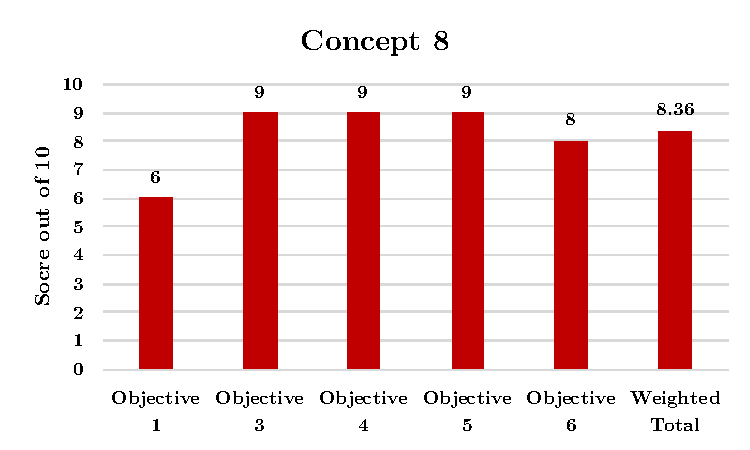
\includegraphics[width=0.95\linewidth]{Concepts/Plots/Round2_3.pdf}}
  \caption{Performance Criteria Assessment Results}
  \label{fig:radar1}
\end{subfigure}
\caption{Concept 5 - Commercially Available VTOL UAV}
\label{fig:concept2}
\end{figure}

\begin{figure}[H]
    \centering
    \fbox{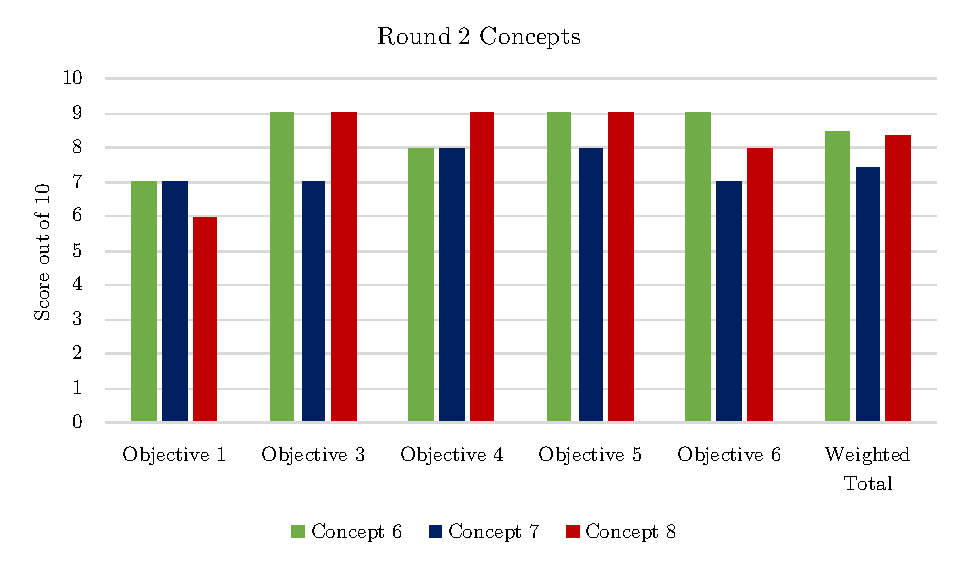
\includegraphics[width = \textwidth]{Concepts/Plots/Round2.pdf}}
    \caption{Summary of Design for Objectives evaluation and scoring for Round 1 Concepts}
    \label{fig:summary}
\end{figure}


\subsection{Round 3 Concepts}
\note{Rhys}{Concepts developed for LM - already done}

\subsection{Final Concept}
\note{Rhys}{Final concept that we present to Craig - [Harry]}

\subsection{Concept Generation Approach Performance}

Figure \ref{fig:improvement} shows the amount of improvement based on performance criteria scores after each round of concept generation.

\begin{figure}[H]
    \centering
    \fbox{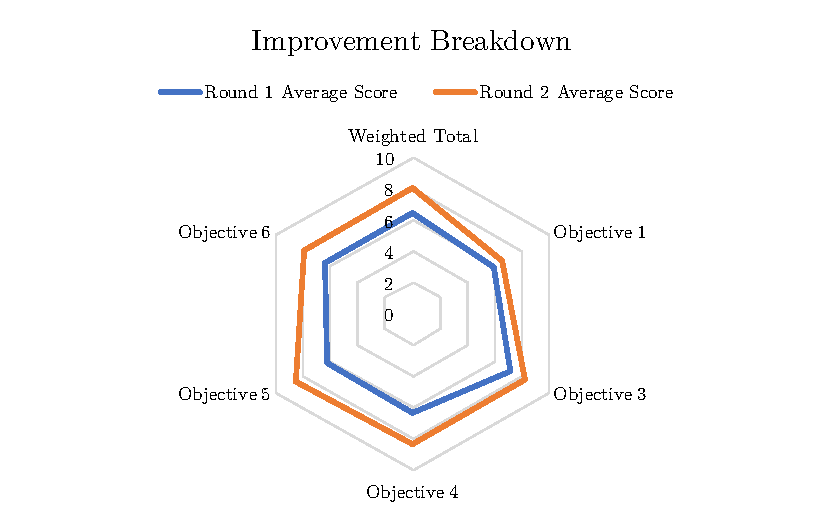
\includegraphics[width = 0.8\textwidth]{Concepts/Improvement.pdf}}
    \caption{Improvement achieved during concept generation rounds}
    \label{fig:improvement}
\end{figure}

